\chapter{狭义相对论中的向量分析}
\label{chap2}

\section{向量的定义}
\label{sec2.1}
我们暂时采用欧几里得几何的向量定义:向量的分量在坐标变换下与坐标的变换规律相同。后面会用更好的方式定义向量。

\textbf{最典型的向量}是位移向量,它从一个事件指向另一事件,分量等于事件的坐标差:
\begin{shaded}
\begin{equation}
    \Delta \vec{x} \xrightarrow[\MO]{ } (\Delta t, \Delta x, \Delta y, \Delta z).
\label{equ2.1}
\end{equation}
\end{shaded}
上式引入了一些新记号:向量用符号之上的箭头表示(例如$\vec{x}$表示一个向量,它与坐标$x$没有特殊关系),$\Delta \vec{x}$之后的右箭头意味着“具有分量”,右箭头下方的$\MO$意味着“在坐标系$\MO$”,坐标的顺序总是$t, x, y, z$(对应于数字指标$0, 1, 2, 3$)。符号$\xrightarrow[\MO]{ }$是为了强调区别向量本身与向量分量。向量$\Delta \vec{x}$是两事件之间的箭头,而向量分量是一组四个依赖于坐标系的数字。为了强调向量(以及之后的张量)的概念,我们称它们为\textbf{几何对象 (geometrical object)}:也就是不依赖于特定坐标系定义的东西。另一种重要的记号是
\begin{equation}
    \Delta \vec{x} \xrightarrow[\MO]{ } \{ \Delta x^\alpha \},
\label{equ2.2}
\end{equation}
其中$\{ \Delta x^\alpha \}$代表所有$\Delta x^0, \Delta x^1, \Delta x^2, \Delta x^3$。为了表示这个向量在另一个坐标系$\MObar$的分量,我们写为
\[
    \Delta \vec{x} \xrightarrow[\MObar]{ }  \{\Delta x^{\bar{\alpha}} \}.
\]
也就是带bar的坐标系对应的分量指标上面也带bar。向量$\Delta \vec{x}$自身是\textbf{不变的},不需要随着更换坐标系而采用新记号,只有分量需要改变。\footnote{这是有些线性代数教材所说的“被动”变换:坐标改变了,而向量没变。} 新分量$\Delta x^{\bar{\alpha}}$\textbf{等于什么}?利用Lorentz变换可以求出它们:
\[
    \Delta x^{\bar{0}} = \frac{\Delta x^0}{\sqrt{1 - v^2}} - \frac{v \Delta x^1}{\sqrt{1 - v^2}}, \text{\ 等等。}
\]
Lorentz变换是线性的,上式可以写为
\[
    \Delta x^{\bar{0}} = \sum_{\beta = 0}^3 \Lambda\indices{^{\bar{0}}_\beta} \Delta x^{\beta},
\]
其中$\{ \Lambda\indices{^{\bar{0}}_\beta} \}$表示四个数,对应于$\beta$取0123,在上述情形中
\begin{align*}
    \Lambda\indices{^{\bar{0}}_0} &= \frac{1}{\sqrt{1 - v^2}}, \quad \Lambda\indices{^{\bar{0}}_1} = -\frac{v}{\sqrt{1 - v^2}}, \\
    \Lambda\indices{^{\bar{0}}_2} &= \Lambda\indices{^{\bar{0}}_3} = 0.
\end{align*}
$\Delta x^{\bar{1}}$以及其它分量同理可得,这些结果可以表示为
\begin{equation}
    \Delta x^{\bar{\alpha}} = \sum_{\beta = 0}^3 \Lambda\indices{^{\bar{\alpha}}_\beta} \Delta x^\beta, \quad \forall\, \bar{\alpha}.
\label{equ2.3}
\end{equation}
其中$\{ \Lambda\indices{^{\bar{\alpha}}_\beta} \}$是16个数的集合,它们是Lorentz变换的矩阵元,把指标写成上下并且错开的理由在之后学习微分几何的时候就会看到。下面来引入最后一个新记号——\textbf{爱因斯坦求和约定}:如果一个表达式含有\textbf{相同的}上下标,则自动意味着对该指标求和。例如
\[
    A_\alpha B^\alpha \quad \text{和} \quad T^\gamma E_{\gamma \alpha}
\]
是如下求和式的简写:
\[
    \sum_{\alpha = 0}^3 A_\alpha B^\alpha \quad \text{和} \quad \sum_{\gamma = 0}^3 T^\gamma E_{\gamma \alpha}.
\]
而
\[
    A_\alpha B^\beta, T^\gamma E_{\beta \alpha}, A_\beta A_\beta
\]
\textbf{不表示}对任何指标的求和。Lorentz变换\eqref{equ2.3}式简写为
\begin{shaded}
\begin{equation}
    \Delta x^{\bar{\alpha}} = \Lambda\indices{^{\bar{\alpha}}_{\beta}} \Delta x^\beta,
\label{equ2.4}
\end{equation}
\end{shaded}
这省了很多麻烦。

注意\eqref{equ2.4}式同样可以写为
\[
    \Delta x^{\bar{\alpha}} = \Lambda\indices{^{\bar{\alpha}}_{\gamma}} \Delta x^\gamma,
\]
因为只要是重复的上下指标(不论是$\beta$还是$\gamma$)都代表从0到3的求和,重复的指标本身是什么无所谓。这种重复表示求和的指标称为\textbf{哑指标 (dummy index)}(又称为\textbf{傀儡指标}),重命名哑指标(例如上面把$\beta$换成$\gamma$)是张量代数的常用技巧。注意不能用\textbf{拉丁字母}替换$\beta$,因为我们约定重复的拉丁字母指标表示对指标$1, 2, 3$(空间部分)求和,而重复的希腊字母(例如$\beta$)表示对所有指标$0, 1, 2, 3$求和。因此,表达式
\[
    \Lambda\indices{^{\bar{\alpha}}_\beta} \Delta x^\beta \text{和} \Lambda\indices{^{\bar{\alpha}}_i} \Delta x^i
\]
并不相同,实际上
\begin{shaded}
\begin{equation}
    \Lambda\indices{^{\bar{\alpha}}_\beta} \Delta x^\beta  = \Lambda\indices{^{\bar{\alpha}}_0} \Delta x^0 +  \Lambda\indices{^{\bar{\alpha}}_i} \Delta x^i.
\label{equ2.5}
\end{equation}
\end{shaded}

\eqref{equ2.4}式表示了4个方程,对应于$\bar{\alpha} = 0, 1, 2, 3$。像$\bar{\alpha}$这样不进行求和的指标称为\textbf{自由指标 (free index)}。一个含有自由指标的方程只有对自由指标的\textbf{每个取值}都成立的时候才成立。与哑指标相似,自由指标也比较自由,例如\eqref{equ2.4}式可以写为
\begin{equation*}
    \Delta x^{\bar{\gamma}} = \Lambda\indices{^{\bar{\gamma}}_{\beta}} \Delta x^\beta,
\end{equation*}
上式与\eqref{equ2.4}式相同,因为$\bar{\gamma}, \bar{\alpha}$都有四个取值都表示四个方程。如果方程中一处的自由指标改变了,则处处都要改变,例如\eqref{equ2.4}式的如下修改是错误的:
\begin{equation*}
    \Delta x^{\bar{\gamma}} = \Lambda\indices{^{\bar{\alpha}}_{\beta}} \Delta x^\beta,
\end{equation*}
以上两式的差别在于,前者保证了无论$\bar{\gamma}$取什么值,等号两侧的$\Delta x^{\bar{\gamma}}$和$\Lambda\indices{^{\bar{\gamma}}_\beta}$总是对应\textbf{相同的}自由指标。第二的式子没有这种关系,因此它与\eqref{equ2.4}式不一样。

一般地,\textbf{向量 (vector)}\footnote{这种有四个分量的向量有时称为\textbf{四维向量}以区分三维空间的三维向量。除非特别指出,我们所说的“向量”都是指四维向量,我们用箭头表示四维向量,例如$\vec{A}$,而用斜黑体表示三维向量,例如$\bm{A}$. }(在坐标系$\MO$的分量)定义为一组数:
\begin{equation}
    \vec{A} \xrightarrow[\MO]{ } (A^0, A^1, A^2, A^3) = \{ A^\alpha \},
\label{equ2.6}
\end{equation}
并且向量分量的变换规律与坐标的变换规律相同,向量在$\MObar$系的分量的满足:
\begin{equation}
    A^{\bar{\alpha}} = \Lambda\indices{^{\bar{\alpha}}_\beta} A^{\beta}.
\label{equ2.7}
\end{equation}

向量可以在某个坐标系中给定四个数字(例如$(10^8, -10^{-16}, 5.8368, \pi)$)来定义;给定了一个坐标系的分量之后,该向量在其它坐标系的分量也唯一确定。时空中的向量服从通常的运算规则:如果$\vec{A}, \vec{B}$是向量,$\mu$是常数,则$\vec{A} + \vec{B}$与$\mu \vec{A}$都是向量,它们的分量分别为
\begin{equation}
\left.
\begin{split}
    \vec{A} + \vec{B} &\xrightarrow[\MO]{ } (A^0+B^0, A^1+B^1, A^2+B^2, A^3+B^3), \\
    \mu \vec{A} &\xrightarrow[\MO]{ } (\mu A^0, \mu A^1, \mu A^2, \mu A^3).
\end{split}
\right\}
\label{equ2.8}
\end{equation}
即向量按照通常的平行四边形法则相加。注意在一个坐标系给定四个数就定义了一个向量,如果这些数具有量纲,则它们的量纲必须相等,这样才能够在坐标变换时相加。


\section{向量代数}
\label{sec2.2}

\subsection*{基向量}
任意惯性系$\MO$都有4个特别的向量,利用它们在$\MO$系的分量进行定义:
\begin{equation}
\left.
\begin{split}
    \vec{e}_0 &\xrightarrow[\MO]{ } (1, 0, 0, 0), \\
    \vec{e}_1 &\xrightarrow[\MO]{ } (0, 1, 0, 0), \\
    \vec{e}_2 &\xrightarrow[\MO]{ } (0, 0, 1, 0), \\
    \vec{e}_3 &\xrightarrow[\MO]{ } (0, 0, 0, 1). \\
\end{split}
\right\}
\label{equ2.9}
\end{equation}
它们是坐标系$\MO$的基向量。类似地,$\MObar$系的基向量为
\[
    \vec{e}_{\bar{0}} \xrightarrow[\MObar]{ } (1, 0, 0, 0), \text{等等。}
\]
一般而言$\vec{e}_{\bar{0}} \neq \vec{e}_0$,因为它们在不同的坐标系定义。读者不难验证上述基向量的定义等价于
\begin{equation}
    (\vec{e}_\alpha)^\beta = \delta\indices{_\alpha^\beta}.
\label{equ2.10}
\end{equation}
也就是说,$\vec{e}_\alpha$的$\beta$分量是Kronecker $\delta$符号:如果$\beta = \alpha$则为1,如果$\beta \neq \alpha$则为0。

任何向量可以表示为基向量的线性组合,任意向量$\vec{A}$在$\MO$系的分量为
\[
    \vec{A} \xrightarrow[\MO]{ } (A^0, A^1, A^2, A^3),
\]
则
\begin{shaded}
\begin{align}
    \vec{A} &= A^0 \Ve_0 + A^1 \Ve_1 + A^2 \Ve_2 + A^3 \Ve_3, \notag \\
    \vec{A} &= A^\alpha \Ve_\alpha. \label{equ2.11}
\end{align}
\end{shaded}
其中最后一行利用了求和约定($\Ve$的指标是\textbf{下标}正是为此)。\eqref{equ2.11}式的含义是向量$\vec{A}$是四个向量$A^0 \Ve_0, A^1 \Ve_1, \dots$的线性和。


\subsection*{基向量的变换}
\eqref{equ2.11}式对任意坐标系都成立,在$\MObar$系中:
\[
    \vec{A} = A^{\bar{\alpha}} \Ve_{\bar{\alpha}}.
\]
这意味着$\vec{A}$也是四个向量$A^{\bar{0}} \Ve_{\bar{0}}, A^{\bar{1}} \Ve_{\bar{1}}, \dots$之和,这四个向量与\eqref{equ2.11}式中的四个向量不同,因为它们与$\MObar$系的基向量平行而非与$\MO$系的基向量平行。尽管不同,但是它们的和等于同一个向量$\vec{A}$。注意,$A^\alpha \Ve_\alpha$与$A^{\bar{\alpha}} \Ve_{\bar{\alpha}}$并非简单地重命名哑指标,带bar与不带bar的指标不能互换,因为它们的含义不同。$\{ A^{\bar{\alpha}}\}$与$\{ A^\alpha \}$不同的两组数,就像$\{ \Ve_{\bar{\alpha}} \}$与$\{ \Ve_\alpha \}$是两组不同的向量那样。但是,根据定义,它们的和相同:
\begin{equation}
    A^\alpha \vec{e}_\alpha = A^{\bar{\alpha}} \Ve_{\bar{\alpha}},
\label{equ2.12}
\end{equation}
上式有一个重要推论:从它可以导出基向量的变换规律,也就是$\{ \Ve_{\bar{\alpha}} \}$与$\{ \Ve_\alpha \}$之间的关系。利用\eqref{equ2.7}式可以将\eqref{equ2.12}写为
\[
    \Lambda\indices{^{\bar{\alpha}}_\beta} A^\beta \Ve_{\bar{\alpha}} = A^\alpha \Ve_\alpha.   
\]
等号左侧进行了\textbf{两次}求和。因为求和的各项都是有限的,因此求和次序无所谓。而由于$\Lambda\indices{^{\bar{\alpha}}_\beta}$和$A^\beta$\textbf{都只是}数字,因此它们的顺序可以改变,上式可以写为
\[
    A^\beta  \Lambda\indices{^{\bar{\alpha}}_\beta} \Ve_{\bar{\alpha}} = A^\alpha \Ve_\alpha.
\]
$\beta$和$\bar{\alpha}$都是哑指标,可以把$\beta$换成$\alpha$,$\bar{\alpha}$换成$\bar{\beta}$:
\[
    A^\alpha  \Lambda\indices{^{\bar{\beta}}_\alpha} \Ve_{\bar{\beta}} = A^\alpha \Ve_\alpha.
\]
上式化为
\[
    A^\alpha (\Lambda\indices{^{\bar{\beta}}_{\alpha}} \Ve_{\bar{\beta}} - \Ve_\alpha ) = 0,
\]
$\vec{A}$是任意向量,上式对所有$\{A^\alpha\}$都成立,由此可得
\[
    \Lambda\indices{^{\bar{\beta}}_{\alpha}} \Ve_{\bar{\beta}} - \Ve_\alpha = 0, \quad \forall\, \alpha,
\]
或者写成
\begin{shaded}
\begin{equation}
    \Ve_\alpha = \Lambda\indices{^{\bar{\beta}}_\alpha} \Ve_{\bar{\beta}}.
\label{equ2.13}
\end{equation}
\end{shaded}
这就是基向量的在坐标变换下的变换规律。它\textbf{不同于}向量分量的变换律:上式将$\MO$系的基向量$\{ \Ve_\alpha \}$表示为$\MObar$系的基向量$\{ \Ve_{\bar{\alpha}} \}$的线性组合。上式与\eqref{equ2.7}式
\[
    A^{\bar{\alpha}} = \Lambda\indices{^{\bar{\alpha}}_\beta} A^{\beta}
\]
比较可得,它们确实不一样。

上面的推导过程使用了一些新技巧,读者应该仔细掌握。注意求和规则省略了求和符号使得方程很整洁。还要注意推导过程的关键步骤在于哑指标重命名:它将彼此孤立的任意向量分量$A^\alpha$与方程的其余内容联系起来。

\subsection*{例}
设$\MObar$系相对于$\MO$系以速度$v$沿$x$轴运动,Lorentz变换矩阵$[\Lambda\indices{^{\bar{\beta}}_{\alpha}}]$为
\[
    (\Lambda\indices{^{\bar{\beta}}_{\alpha}}) = 
    \begin{pmatrix}
        \gamma & -v\gamma & 0 & 0 \\
        -v \gamma & \gamma & 0 & 0 \\
        0 & 0 & 1 & 0 \\
        0 & 0 & 0 & 1
    \end{pmatrix},
\]
其中利用了标准记号
\[
    \gamma := \frac{1}{\sqrt{1 - v^2}}.
\]
如果$\vec{A} \xrightarrow[\MO]{ } (5, 0, 0, 2)$,则$\vec{A}$在$\MObar$系的分量为:
\begin{align*}
    A^{\bar{0}} &= \Lambda\indices{^{\bar{0}}_0} A^0 + \Lambda\indices{^{\bar{0}}_1} A^1 + \dots \\
    &= \gamma \cdot 5 + (-v \gamma) \cdot 0 + 0 \cdot 0 + 0 \cdot 2 \\
    &= 5\gamma.
\end{align*}
类似地可以算出
\begin{align*}
    A^{\bar{1}} &= -5v\gamma, \\
    A^{\bar{2}} &= 0, \\
    A^{\bar{3}} &= 2.
\end{align*}
因此$\vec{A} \xrightarrow[\MObar]{ } (5\gamma, -5v\gamma, 0, 2)$.

基向量的变换律是
\[
    \Ve_\alpha = \Lambda\indices{^{\bar{\beta}}_\alpha} \Ve_{\bar{\beta}},
\]
或者展开写成
\begin{align*}
    \Ve_0 &= \Lambda\indices{^{\bar{0}}_0} \Ve_{\bar{0}} + \Lambda\indices{^{\bar{1}}_{0}} \Ve_{\bar{1}} + \dots \\
    &= \gamma \Ve_{\bar{0}} - v \gamma \Ve_{\bar{1}}.
\end{align*}
类似可得
\begin{align*}
    \Ve_1 &= -v \gamma Ve_{\bar{0}} + \gamma \Ve_{\bar{1}}, \\
    \Ve_2 &= \Ve_{\bar{2}}, \\
    \Ve_3 &= \Ve_{\bar{3}}.
\end{align*}
这样用$\MObar$系的基向量表示了$\MO$的基向量。我们在$\MObar$系中画出了示意图(如图\ref{fig2.1}):变换律保证了变换后的基向量沿着相应的坐标轴,可以将图\ref{fig2.1}与图1.5(b)进行比较。

{
    \centering
    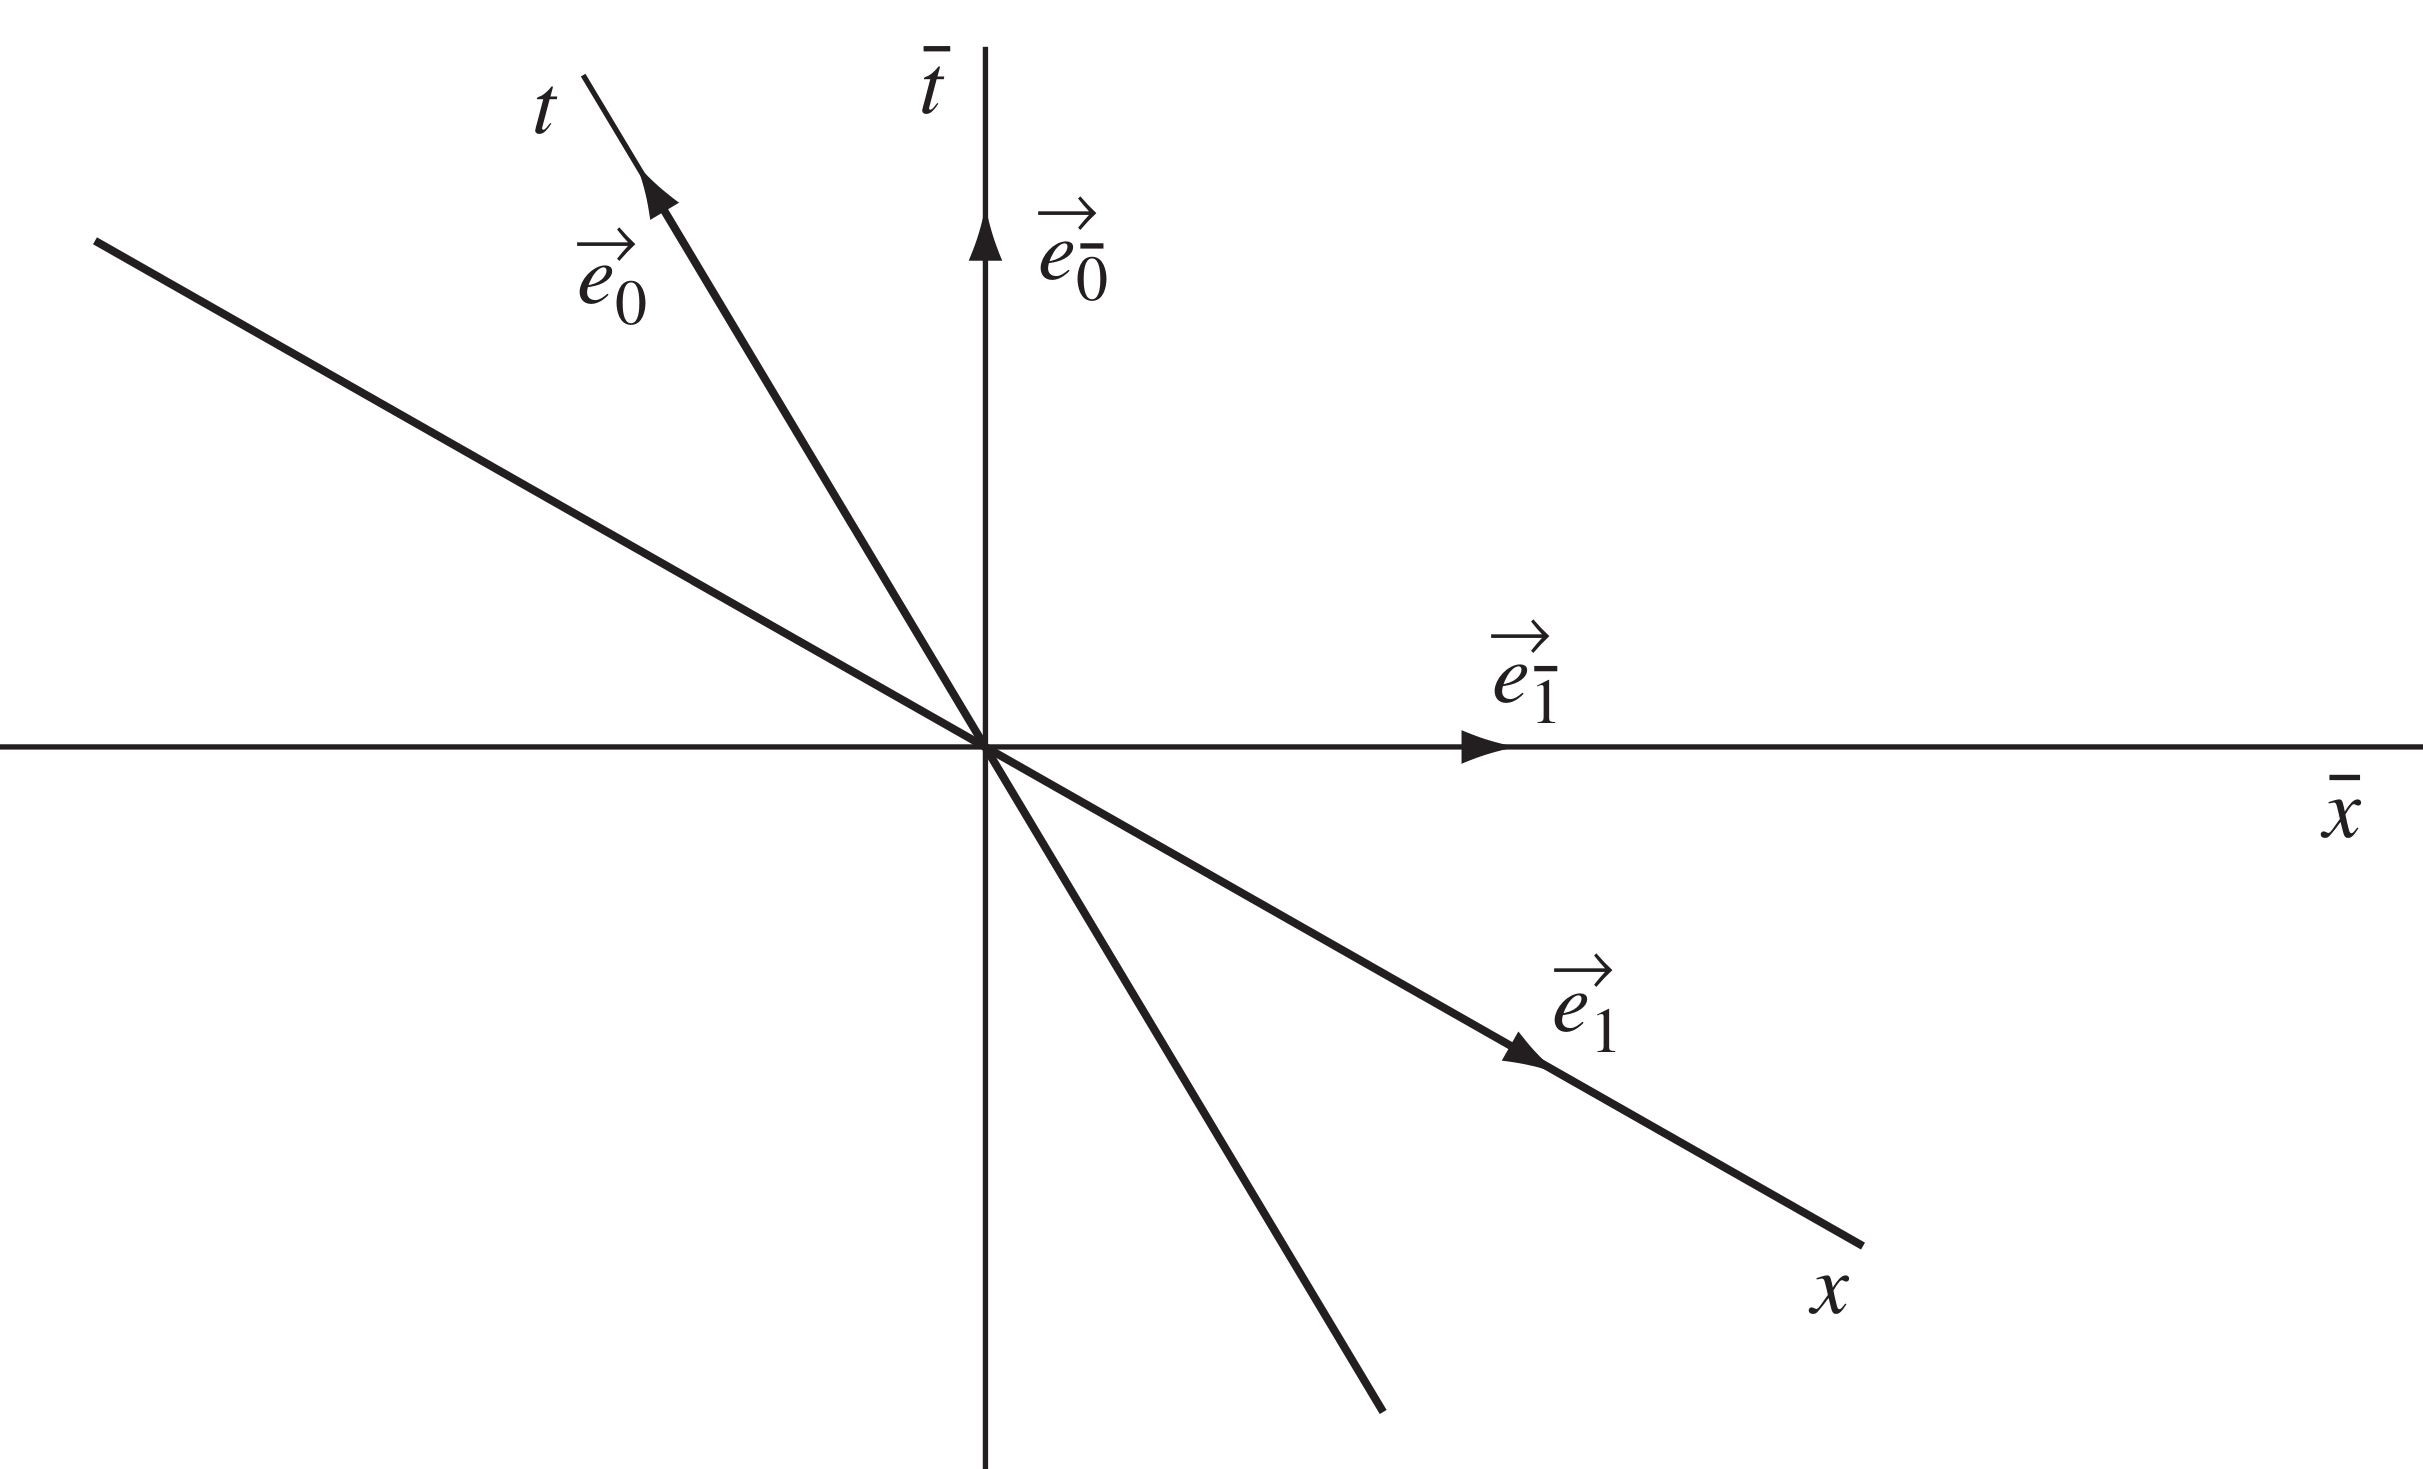
\includegraphics[width=0.7\textwidth]{fig2.1.png}
    \figcaption{\textit{ 在$\MObar$系中画出$\MO$系和$\MObar$系的基向量。 }}
    \label{fig2.1}
}



\subsection*{逆变换}
洛伦兹变换$\Lambda\indices{^{\bar{\beta}}_\alpha}$只依赖于两个坐标系之间的相对速度,下面将这种依赖关系写明:
\[
    \Lambda\indices{^{\bar{\beta}}_\alpha} = \Lambda\indices{^{\bar{\beta}}_\alpha} (\bm{v}).
\]
于是
\begin{equation}
    \Ve_\alpha = \Lambda\indices{^{\bar{\beta}}_\alpha} (\bm{v})\, \Ve_{\bar{\beta}}.
\label{equ2.14}
\end{equation}
如果$\MO$的基向量是通过$\MObar$的基向量经过速度$\bm{v}$对应的Lorentz变换得到的,那么逆变换必然是$(-\bm{v})$对应的,即:
\begin{equation}
    \Ve_{\bar{\mu}} = \Lambda\indices{^\nu_{\bar{\mu}}}(-\bm{v}) \, \Ve_\nu.
\label{equ2.15}
\end{equation}
上式采用新的$\bar{\mu}, \nu$以避免与上上式混淆,带bar的指标仍然是指$\MObar$系。矩阵$[\Lambda\indices{^\nu_{\bar{\mu}}}]$是矩阵$[\Lambda\indices{^{\bar{\beta}}_\alpha}]$将$\bm{v}$替换成$-\bm{v}$得到的。指标上的bar只是用来\textbf{标记}观测者:变换矩阵$[\Lambda]$相应的速度($\bm{v}$或者$-\bm{v}$)\textbf{总是}\textit{上标对应的坐标系}相对于\textit{下标对应的坐标系}的速度。这在\eqref{equ2.14}和\eqref{equ2.15}式特别清楚,$\bm{v}$是$\MObar$系(\eqref{equ2.14})式的上标坐标系)相对于$\MO$系的速度;而$-\bm{v}$是$\MO$系(\eqref{equ2.15}式的上标坐标系)相对于$\MObar$系的速度。本章习题11帮助读者进一步理解这一点。

\eqref{equ2.15}式可以写为
\[
    \Ve_{\bar{\beta}} = \Lambda\indices{^\nu_{\bar{\beta}}}(-\bm{v}) \, \Ve_\nu.
\]
上式只是把$\bar{\mu}$替换成了$\bar{\beta}$,方程的含义没有任何改变,同样是$\bar{\beta}$的四个值对应四个方程。上式带入$\Ve_\alpha$的表达式\eqref{equ2.14}式中:
\begin{equation}
    \Ve_\alpha = \Lambda\indices{^{\bar{\beta}}_\alpha}(\bm{v}) \, \Ve_{\bar{\beta}} = \Lambda\indices{^{\bar{\beta}}_\alpha}(\bm{v}) \Lambda\indices{^\nu_{\bar{\beta}}}(-\bm{v}) \, \Ve_\nu.
\label{equ2.16}
\end{equation}
上式只出现了$\MO$的基向量。因此它必然是对\textbf{所有}$\bm{v}$成立的恒等式。等式右侧含有两个求和,对$\bar{\beta}$和对$\nu$的。先计算对$\bar{\beta}$的求和,则等号右侧就是$\{ \Ve_\nu \}$的线性组合,每个$\Ve_\nu$对应的线性系数为:
\begin{equation}
    \sum_{\bar{\beta}} \Lambda\indices{^{\bar{\beta}}_\alpha}(\bm{v}) \, \Lambda\indices{^\nu_{\bar{\beta}}} (-\bm{v}).
\label{equ2.17}
\end{equation}
考虑\eqref{equ2.16}式中的某个固定的$\alpha$,等号成立意味着等号\textbf{右侧}的$\Ve_\alpha$的系数必须为1,而其余系数必须为0。用数学形式表示为
\[
    \Lambda\indices{^{\bar{\beta}}_\alpha}(\bm{v}) \, \Lambda\indices{^\nu_{\bar{\beta}}} (-\bm{v}) = \delta\indices{^\nu_\alpha},
\]
其中$\delta\indices{^\nu_\alpha}$是Kronecker delta符号,这样可以导出
\[
    \Ve_\alpha = \delta\indices{^\nu_\alpha} \Ve_\nu,
\]
它是个恒等式。

更换相乘顺序,将上面的关键公式写为
\begin{shaded}
\begin{equation}
    \Lambda\indices{^\nu_{\bar{\beta}}} (-\bm{v}) \, \Lambda\indices{^{\bar{\beta}}_\alpha}(\bm{v}) = \delta\indices{^\nu_\alpha}.
\label{equ2.18}
\end{equation}
\end{shaded}
上式意味着矩阵$[\Lambda\indices{^\nu_{\bar{\beta}}} (-\bm{v})]$和矩阵$[\Lambda\indices{^{\bar{\beta}}_\alpha}(\bm{v})]$\textbf{互逆},因为对$\bar{\beta}$的求和意味着两个矩阵相乘。矩阵$(\delta\indices{^\nu_\alpha})$就是单位矩阵。

向量分量的变换式
\[
    A^{\bar{\beta}} = \Lambda\indices{^{\bar{\beta}}_\alpha}(\bm{v}) \, A^\alpha,
\]
也有相应的逆形式。等号两侧乘以$\Lambda\indices{^\nu_{\bar{\beta}}} (-\bm{v})$,对$\bar{\beta}$求和:
\begin{align*}
    \Lambda\indices{^\nu_{\bar{\beta}}} (-\bm{v})  \, A^{\bar{\beta}} &= \Lambda\indices{^\nu_{\bar{\beta}}} (-\bm{v}) \, \Lambda\indices{^{\bar{\beta}}_\alpha}(\bm{v}) \, A^\alpha \\
    &= \delta\indices{^\nu_\alpha} A^\alpha \\
    &= A^\nu.
\end{align*}
这意味着$\vec{A}$在$\MO$系的分量等于$\MObar$系的分量经过速度$-\bm{v}$对应的Lorentz变换得到,我们得到了正确结论。

上述内容与读者熟悉的欧几里得空间中的向量代数类似,只是这里采用了新的指标记号,这种记号在本书其余的部分大用特用。读者应该掌握上述内容的几何意义以及代数依据。



\section{四维速度}
\label{sec2.3}
世界线的四维速度(four-velocity, 简称四速)是一种十分重要的向量。伽利略的三维几何中,速度是与粒子运动轨迹相切的向量。四维几何的四维速度$\vec{U}$定义为与粒子世界线相切的、在粒子的参考系中长度为单位时间的向量。先考虑最简单的匀速直线运动粒子,在与粒子相对静止的惯性系中,根据定义,四维速度向量的方向与时间轴平行、长度为单位时间,这意味着四维速度就等于该系的基向量$\vec{e}_0$。于是,匀速直线运动粒子的四维速度定义为该粒子静止惯性系的基向量$\vec{e}_0$. “四维速度”名字的来历是$\vec{U}$的空间分量与通常所说的粒子的三维速度$\bm{p}$关系密切,参见下面的例子与\eqref{equ2.21}式。


\textit{变速运动的粒子}不存在始终在其中静止的惯性系。然而,\textit{仍然存在着}与粒子瞬时静止的惯性系——它的速度在一瞬间与粒子速度相同(共动参考系),不过在下一时刻就不再是共动的了。这个参考系称为\textit{瞬时共动参考系 (momentarily comoving reference frame,} \textbf{\ MCRF} \textit{)},这个概念极其重要。(实际上,一个粒子在某一特定事件点有无数个MCRF;它们的速度相同,而空间坐标轴相差旋转变换。不过这通常不重要,取哪个空间轴取向的MCRF都行)变速运动粒子(在某一事件点)的四速\textit{定义为}在该事件点的MCRF的基向量$\vec{e}_0$. 该向量与(弯曲的)粒子世界线相切。图\ref{fig2.2}中,粒子在事件$\mathscr{A}$的MCRF是$\MObar$系,图中画出了基向量,$\vec{e}_{\bar{0}}$就是粒子在$\mathscr{A}$点的四速$\vec{U}$.

{
    \centering
    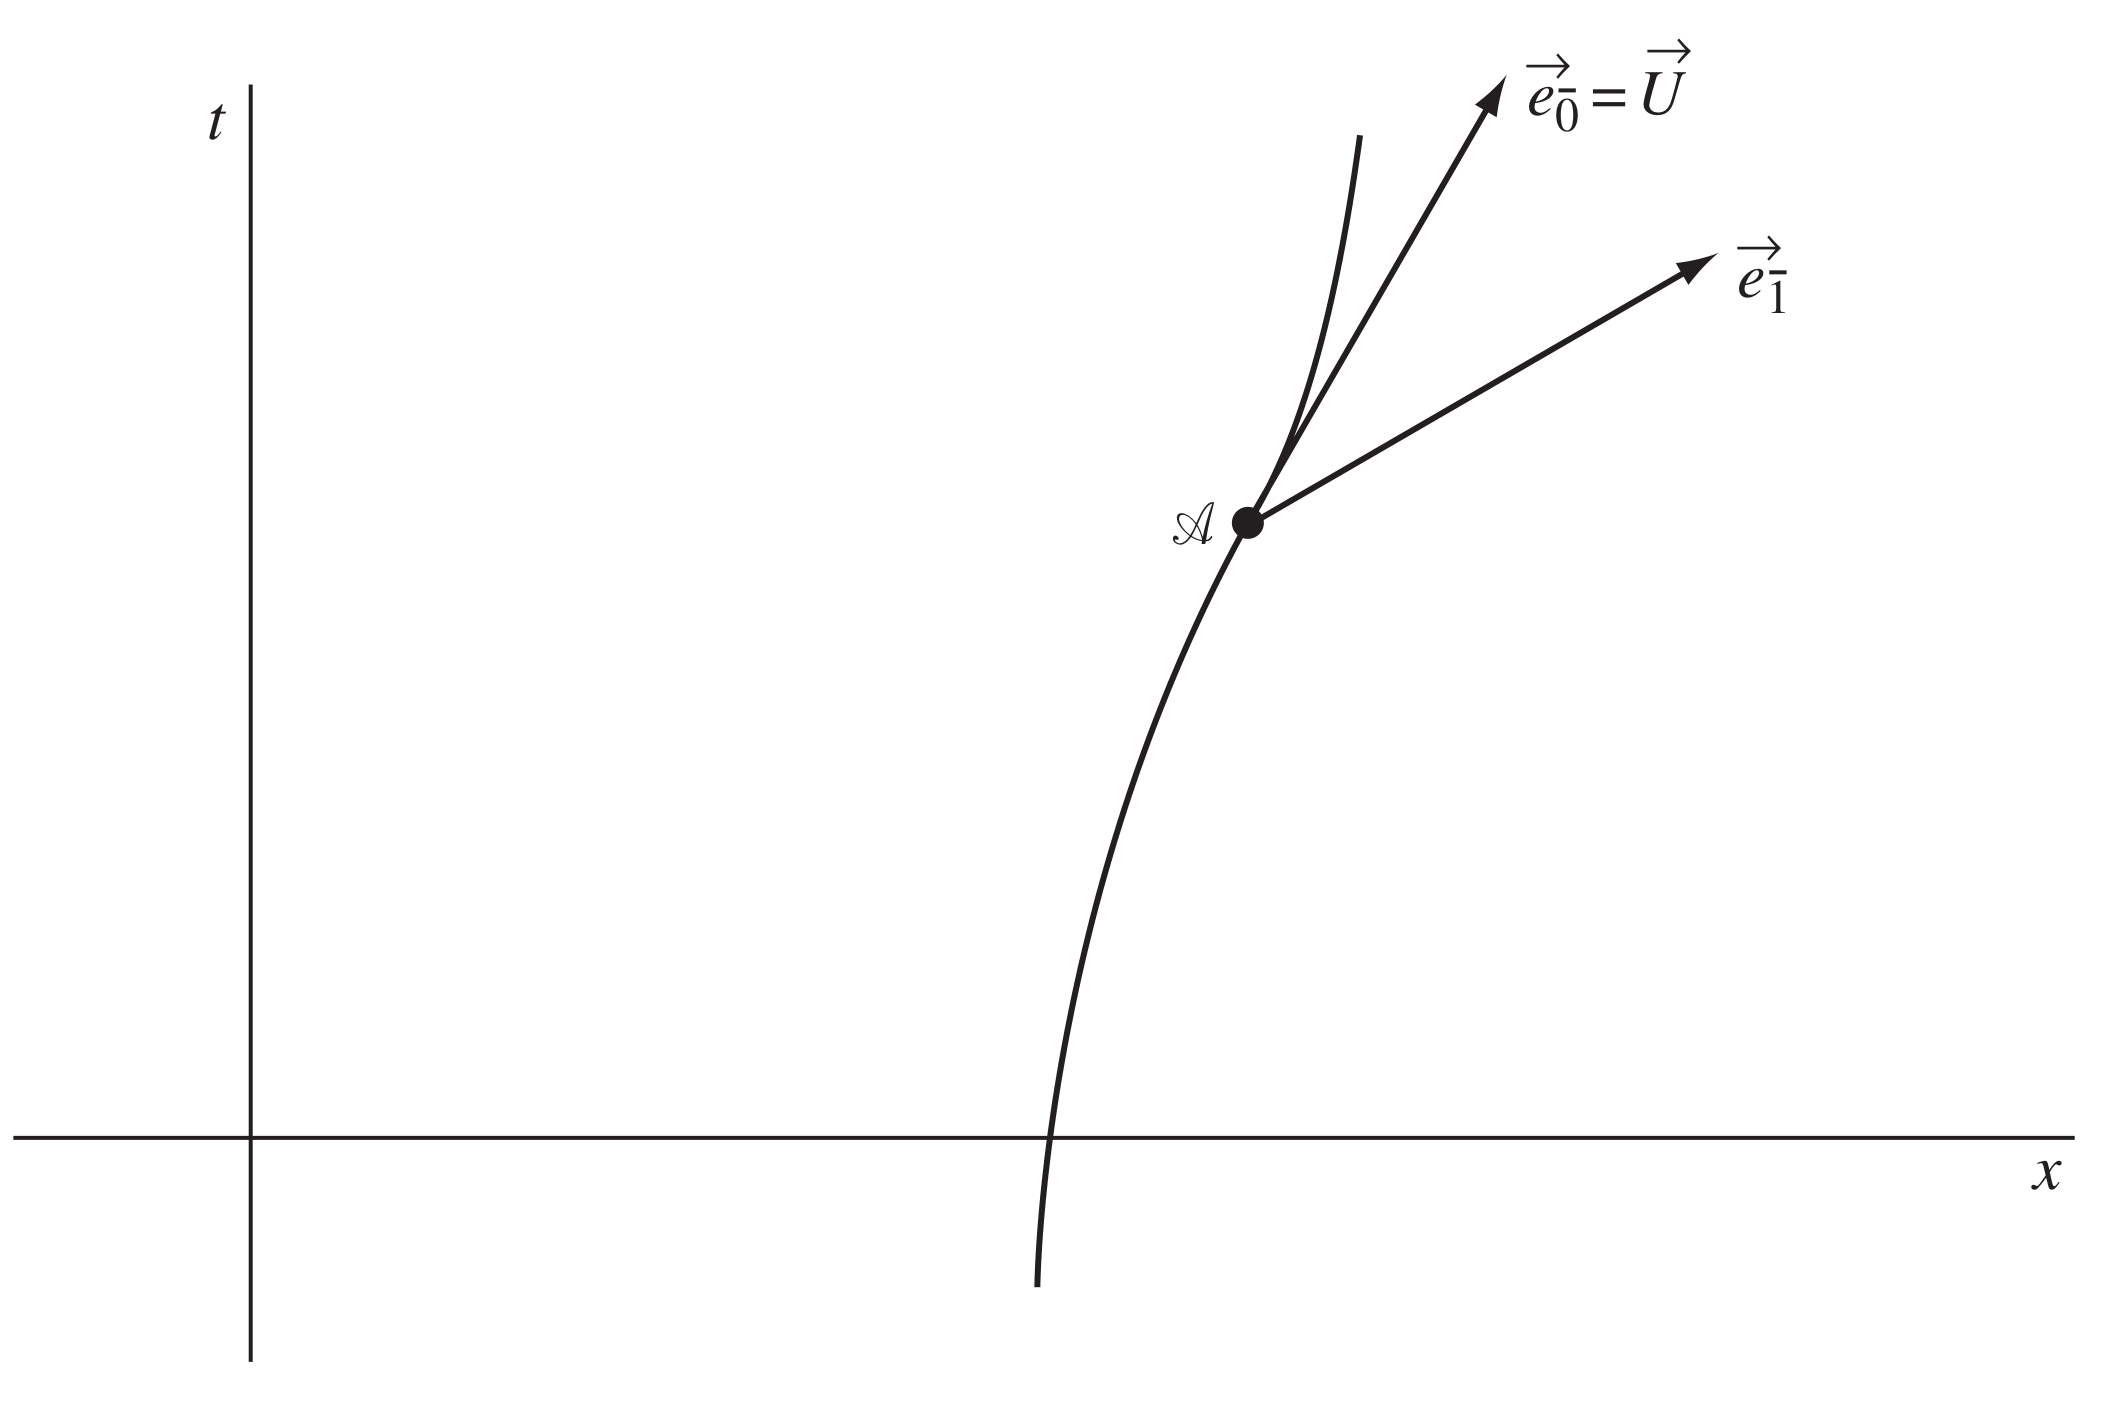
\includegraphics[width=0.7\textwidth]{fig2.2.png}
    \figcaption{\textit{粒子世界线在$\mathscr{A}$点的四维速度与MCRF基向量}}
    \label{fig2.2}
}


\section{四维动量}
\label{sec2.4}
四维动量$\vec{p}$定义为
\begin{shaded}
\begin{equation}
    \vec{p} = m \vec{U},
\label{equ2.19}
\end{equation}
\end{shaded}
其中$m$是粒子的\textit{静止质量 (rest mass,简称静质量)},也就是在粒子静止的坐标系中测得的粒子质量。四动量在任一惯性系$\MO$中的分量记作
\begin{equation}
    \vec{p} \xrightarrow[\MO]{ } (E, p^1, p^2, p^3).
\label{equ2.20}
\end{equation}
分量$p^0$记作$E$,称为粒子在坐标系$\MO$中的\textit{能量 (energy)}。其余分量称为四动量的空间分量$p^i$.

\subsection*{例子}
静质量为$m$的粒子在坐标系$\MO$中沿$x$轴方向运动,速度为$\bm{v}$,粒子四速、四动量在$\MO$系的分量是什么?粒子在其中静止的坐标系记作$\MObar$,该系的时间基向量为$\vec{e}_{\bar{0}}$。根据四速与四动量的定义有
\begin{equation}
\begin{split}
    \vec{U} &= \vec{e}_{\bar{0}}, & \quad \vec{p} &= m\vec{U}, \\
    U^\alpha &= \Lambda\indices{^\alpha_{\bar{\beta}}} ( \vec{e}_{\bar{0}} )^{\bar{\beta}} = \Lambda\indices{^\alpha_{\bar{0}}}, \quad & p^\alpha &= m \Lambda\indices{^\alpha_{\bar{0}}}.
\end{split}
\label{equ2.21}
\end{equation}
由此可得
\begin{align*}
    U^0 &= (1 - v^2)^{-1/2}, \quad & p^0 &= m(1 - v^2)^{-1/2}, \\
    U^1 &= v (1 - v^2)^{-1/2}, \quad & p^1 &= mv (1 - v^2)^{-1/2}, \\
    U^2 &= 0, \quad & p^2 &= 0, \\
    U^3 &= 0, \quad & p^3 &= 0.
\end{align*}
对于很小的$v$,$\vec{U}$的空间分量近似为$(v, 0, 0)$,$\vec{p}$的空间分量为$(mv, 0, 0)$,从这就能看出它们的名字——四维速度、四维动量——的合理性。还是对于很小的$v$,能量近似为:
\begin{equation*}
    E := p^0 = m (1 - v^2)^{-1/2} \approx m + \frac{1}{2} m v^2.
\end{equation*}
它等于静质能(rest-mass energy)与(伽利略形式的)动能之和。

\subsection*{四维动量守恒}
伽利略力学中,粒子的碰撞过程遵从能量、动量守恒定律。因为$\vec{p}$的分量在非相对论极限下退化为伽利略形式的能量、动量,因此很自然地假设在相对论情形下,四维向量$\vec{p}$也守恒。也就是说,几个粒子发生相互作用,粒子的总动量:
\begin{equation}
    \vec{p} := \sum_{\text{所有粒子,编号为}(i)} \vec{p}_{(i)},
\label{equ2.22}
\end{equation}
在碰撞过程的前后不变。($\vec{p}_{(i)}$是第$i$个粒子的动量)

四维动量守恒定律实际上是个额外\textit{假设},因为我们只知道它的非相对论极限是正确的。不过就像SR的两条基本假设那样,四动量守恒经历了丰富的实验验证。至少它预言了能量守恒定律必须包括静质能:静质量可以消灭、相应的能量可以转化为动能从而化为热能。这个预言每天都在被核电站所验证。

上面四动量守恒的陈述中掩藏了很重要的一点:一次碰撞“之前”与“之后”的含义是什么?假设不同的粒子发生了两次碰撞,这两个事件的间隔是类空的,如下图。要将同一时刻的四动量相加,应该沿着等$t$时刻还是等$\bar{t}$时刻?如图\ref{fig2.3}所示,$\MO$系的测量结果为:事件$\mathscr{A}$发生在$t = 0$之前,事件$\mathscr{B}$在之后,因此$t = 0$时刻的总动量等于$\mathscr{A}$之后加上$\mathscr{B}$之前的动量。而在$\MObar$系中,事件$\mathscr{A}, \mathscr{B}$同时发生于时刻$\bar{t} = 0$之前,因此$\bar{t} = 0$时刻的总动量等于事件$\mathscr{A}, \mathscr{B}$之后的动量之和。 甚至还可以找到一个坐标系,在其中事件$\mathscr{B}$比$\mathscr{A}$发生的\textit{更早},and the adding-up may be the reverse of $\MO$'s. 

{
    \centering
    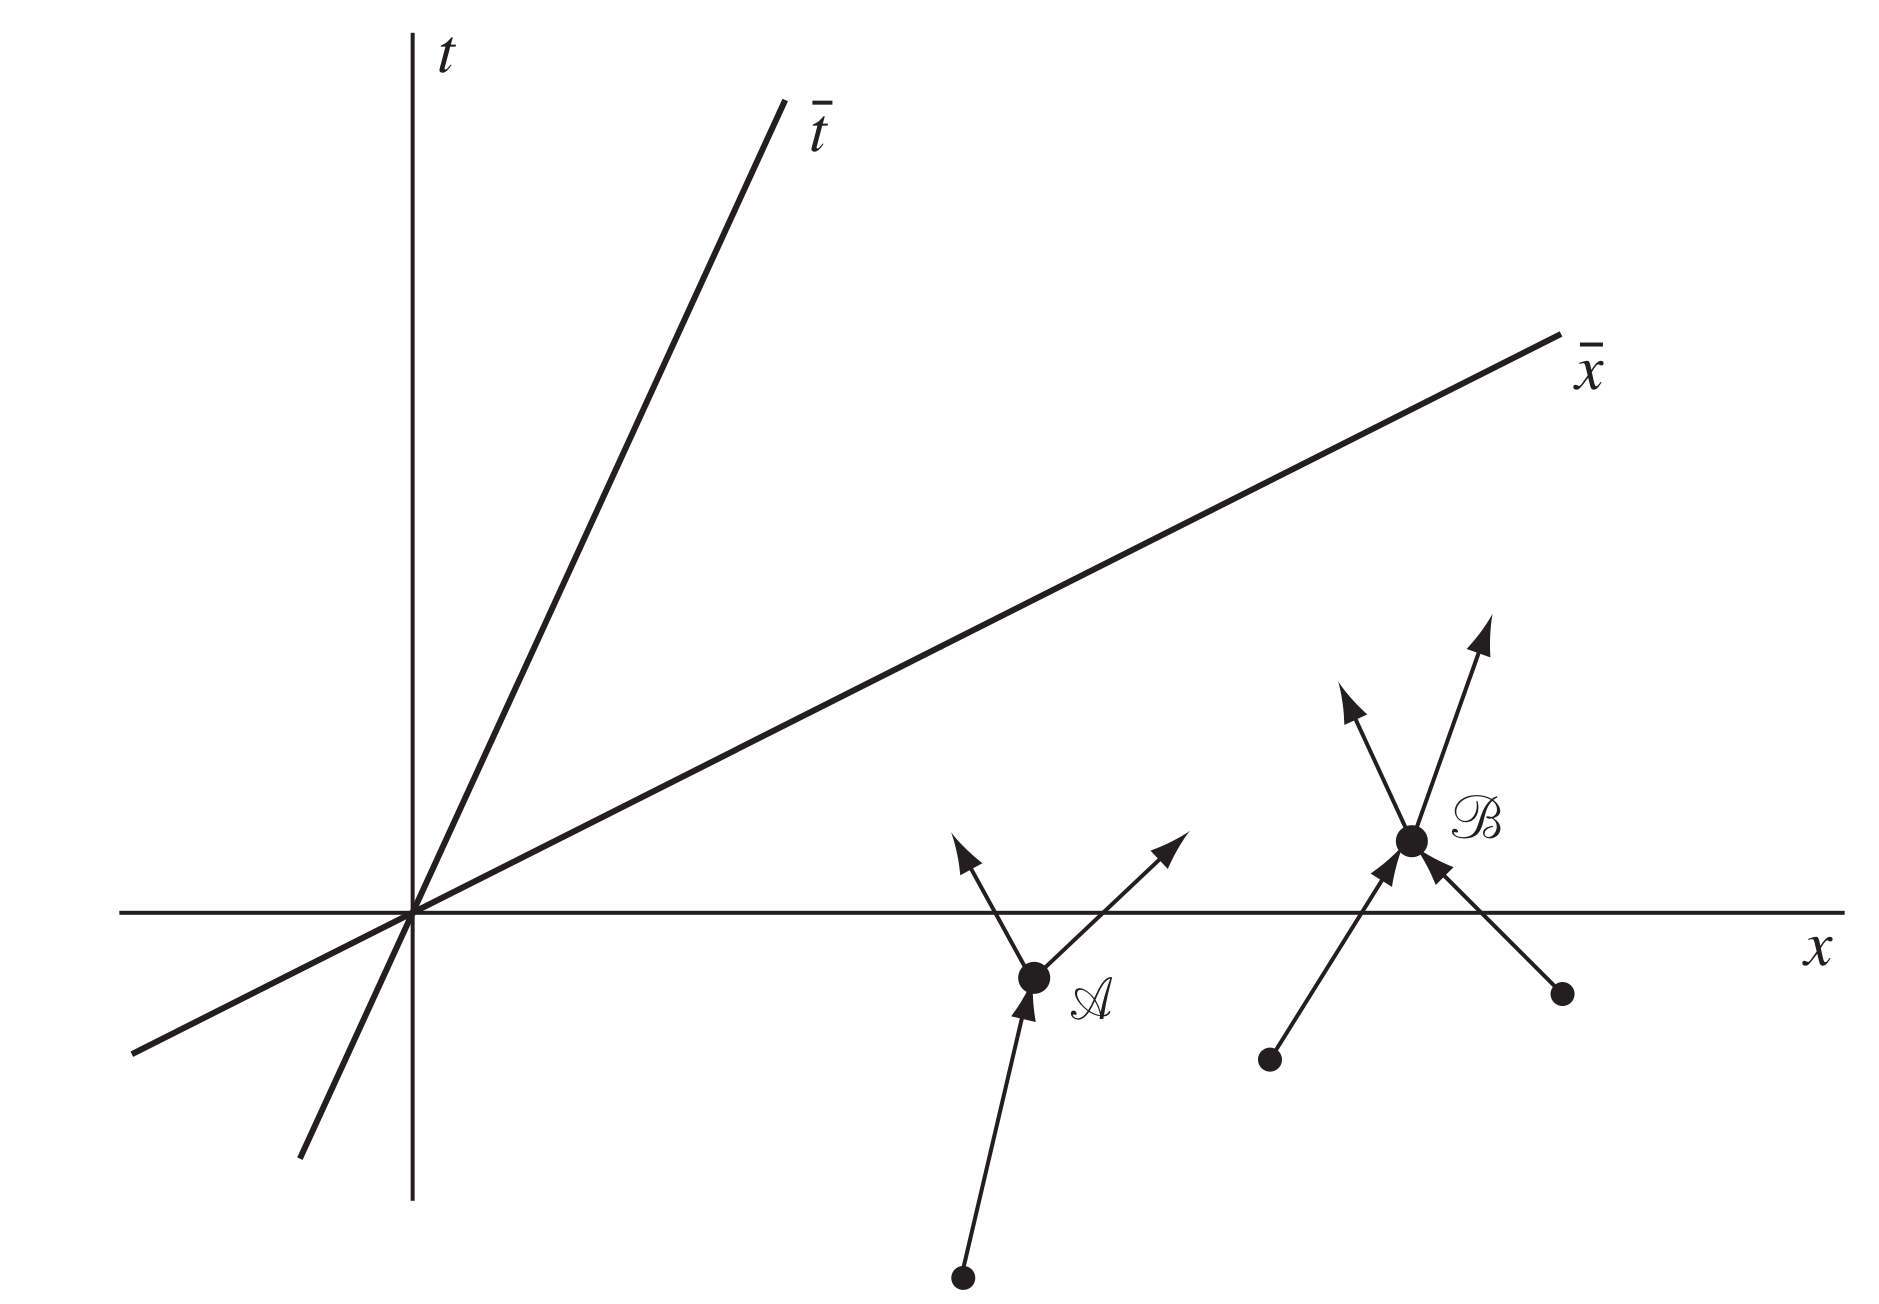
\includegraphics[width=0.7\textwidth]{fig2.3.png}
    \figcaption{\textit{当考虑几个碰撞过程时,组成某一时刻的总动量的各个四动量取决于坐标系,但总的四维动量是在所有坐标系中相同的四维向量;它的分量在坐标系之间的变换规律服从Lorentz变换。}}
    \label{fig2.3}
}

这实际上没问题。既然每个碰撞过程都服从动量守恒,那么事件$\mathscr{A}$之后与之前的动量和相等,事件$\mathscr{B}$也一样。因此\textit{每个}惯性观者都得到相同的总的四动量$\vec{p}$。(它的分量随坐标系的不同而不同,但是它是同一个向量。) 有一点很重要:\textit{任意}观者可以定义他自己的等时线(这实际上是等时的三维空间,称之为四维时空中等时的\textit{超平面}),把那个时刻的所有动量相加,得到的向量与其他任何观者的结果都相同。理解这一点十分重要,因为这种守恒律会在之后再次出现。

\subsection*{质心 (CM) 系}
质心系(center of momentum frame, CM)是总动量的空间分量在其中为零的惯性系:
\begin{equation}
    \sum_i \vec{p}_{(i)} \xrightarrow[\text{CM}]{ } (E_{\text{TOTAL}}, 0, 0, 0).
\label{equ2.23}
\end{equation}
与MCRF同理,任意相对于CM系静止的坐标系也是CM系。

\section{标量积}
\label{sec2.5}

\subsection*{四维向量的模}
类比间隔的定义,四维向量$\vec{A}$的\textit{模 (magnitude)}定义为
\begin{equation}
    \vec{A}^2 = -(A^0)^2 + (A^1)^2 + (A^2)^2 + (A^3)^2.
\label{equ2.24}
\end{equation}
根据向量分量的\textit{定义},向量分量在坐标变换下与$(\Delta t, \Delta x, \Delta y, \Delta z)$的变换规律相同,服从Lorentz变换,这就\textit{保证了}
\begin{equation}
    -(A^0)^2 + (A^1)^2 + (A^2)^2 + (A^3)^2 = -(A^{\bar{0}})^2 + (A^{\bar{1}})^2 + (A^{\bar{2}})^2 + (A^{\bar{3}})^2.
\label{equ2.25}
\end{equation}
向量的模就定义成这样的不依赖于坐标系的量,即Lorentz变换下的标量 (scalar)。

向量模不一定是正数。我们把向量按照间隔那样进行分类:
\begin{itemize}
    \item 如果$\vec{A}^2$是正数,则称$\vec{A}$是\textit{类空 (spacelike)}向量;
    \item 如果$\vec{A}^2$等于零,则称$\vec{A}$是\textit{null}向量\footnote{通译为“零向量”,然而这个名字给人一种\sout{钦定的}所有分量都为零的感觉,事实上并非如此(例如向量$(1, 1, 0, 0)$的模$\big( -(1)^2 + 1^2 \big) = 0$. 因此我们不采用“零向量”的译法,暂时称呼它为“null 向量”。};
    \item 如果$\vec{A}^2$是负数,则称$\vec{A}$是\textit{类时 (timelike)}向量。
\end{itemize}
这样,空间中的向量的模是正数,就像欧几里得空间的情况那样。必须注意,null向量\textit{不同于}zero向量。也就是说,null向量满足$\vec{A}^2 = 0$,但它的所有$A^\alpha$不一定都为零;而zero向量的所有分量都是零。只有在$\vec{A}^2$均为正定(positive-definite)的空间中,$\vec{A}^2 = 0$才意味着$\forall\, \alpha, A^\alpha = 0$.

\subsection*{两个向量的标量积}
向量$\vec{A}, \vec{B}$(在某个惯性系$\MO$)的标量积 (scalar product)定义为
\begin{shaded}
\begin{equation}
    \vec{A} \cdot \vec{B} = -A^0 B^0 + A^1 B^1 + A^2 B^2 + A^3 B^3.
\label{equ2.26}
\end{equation}
\end{shaded}
下面来证明这个标量积在其它惯性系也是同样的值。

首先注意到$\vec{A} \cdot \vec{A}$就是$\vec{A}^2$,我们已经知道后者是个坐标变换下的不变量。因此$(\vec{A} + \vec{B}) \cdot ( \vec{A} + \vec{B} )$,即$\vec{A} + \vec{B}$的模,也是不变量。根据\eqref{equ2.24}和\eqref{equ2.26}式可得
\begin{equation*}
    (\vec{A} + \vec{B}) \cdot ( \vec{A} + \vec{B} ) = \vec{A}^2 + \vec{B}^2 + 2 \vec{A} \cdot \vec{B}.
\end{equation*}
因为等号左侧的项以及右侧的前两项在所有坐标系中相等,因此最后一项也在所有坐标系中相等。这就证明了向量积是坐标系不变量。

如果$\vec{A} \cdot \vec{B} = 0$,则称向量$\vec{A}$与$\vec{B}$\textit{垂直 (orthogonal)}。标量积定义中的负号意味着相互垂直的两个向量不一定非得在时空图中成直角(见下文的例子)。一种极端情况是null向量,它与\textit{自身}垂直!这种现象在标量积是正定的空间中不会出现。

\subsection*{例1}
$\MO$系的基向量满足:
\begin{align*}
    \vec{e}_0 \cdot \vec{e}_0 &= -1, \\
    \vec{e}_1 \cdot \vec{e}_1 &= \vec{e}_2 \cdot \vec{e}_2 = \vec{e}_3 \cdot \vec{e}_3 = +1, \\
    \vec{e}_\alpha \cdot \vec{e}_\beta &= 0, \quad \text{如果} \ \alpha \neq \beta.
\end{align*}
因此它们组成了一组相互正交的向量四元组:一组\textit{规范正交基},这意味着这组基的所有基向量\textit{相互正交}并且\textit{归一化}——具有单位模. (类空向量的“单位模”意味着模为$-1$.)上式可以总结为
\begin{shaded}
\begin{equation}
    \vec{e}_\alpha \cdot \vec{e}_\beta = \eta_{\alpha \beta},
\label{equ2.27}
\end{equation}
\end{shaded}
其中$\eta_{\alpha \beta}$和Kronecker\ $\delta$符号有点像——当$\alpha \neq \beta$时$\eta_{\alpha \beta} = 0$,但有所不同:$\eta_{00} = -1, \eta_{11} = \eta_{22} = \eta_{33} = +1$. 后面会看到$\eta_{\alpha \beta}$的地位极其重要:它是度规张量。不过现在把它当作Kronecker\ $\delta$的推广就好了。

\subsection*{例2}
$\MObar$系的基向量也满足
\begin{equation*}
    \vec{e}_{\bar{\alpha}} \cdot \vec{e}_{\bar{\beta}} = \eta_{\bar{\alpha} \bar{\beta}},
\end{equation*}
因此$\vec{e}_{\bar{0}} \cdot \vec{e}_{\bar{1}} = 0$. 考虑图\ref{fig2.4}中的时空图:图中的$\vec{e}_{\bar{0}}, \vec{e}_{\bar{1}}$看起来不垂直。然而它们的标量积等于零。如果两个向量与$45^\circ$倾斜的直线(光的世界线)的夹角相等,那么这两个向量垂直。因此,与光的世界线相切的向量与自身垂直。这是SR中不能用欧几里得空间类比的又一个概念。

{
    \centering
    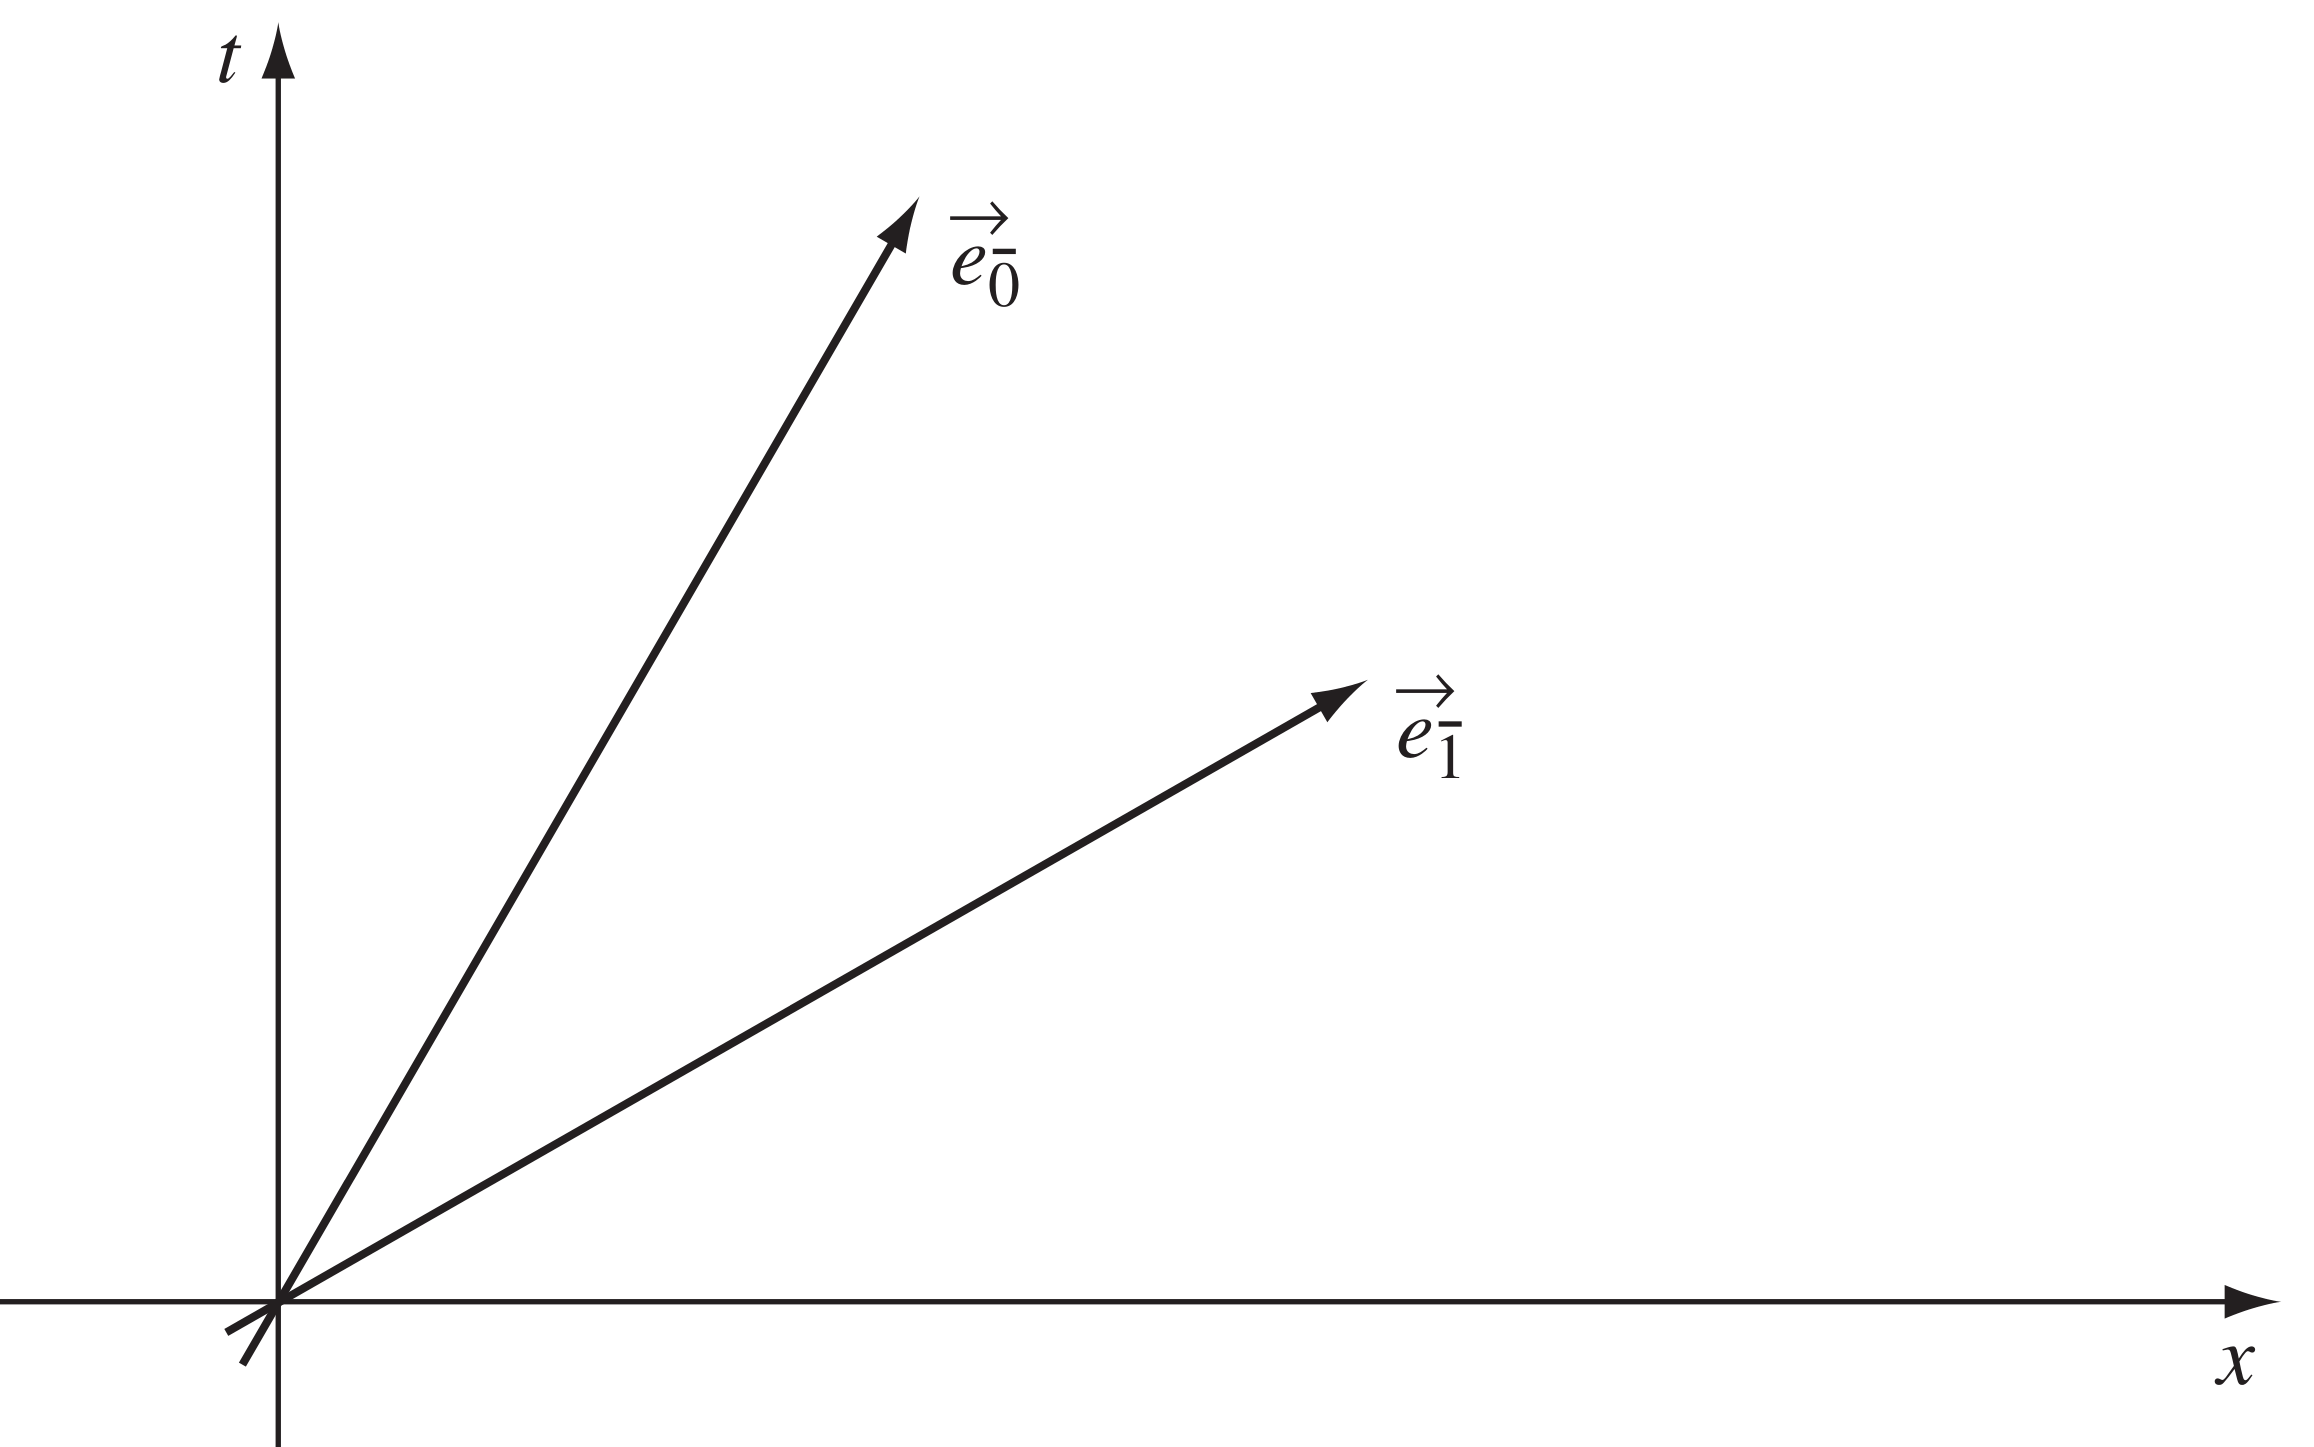
\includegraphics[width=0.5\textwidth]{fig2.4.png}
    \figcaption{\textit{在$\MO$系之下,$\MObar$系的基向量(用欧几里得空间的眼光)看起来并不“垂直”,但是它们在Minkowski时空的向量积定义下却是正交的。}}
    \label{fig2.4}
}

\subsection*{例3}
粒子的四维速度$\vec{U}$就是粒子MCRF的基向量,因此根据\eqref{equ2.27}式可得
\begin{equation}
    \vec{U} \cdot \vec{U} = -1.
\label{equ2.28}
\end{equation}

\section{应用}
\label{sec2.6}

\subsection*{四速与四加速的导数形式}
设粒子进行了无穷小位移$\rd \vec{x}$,$\rd \vec{x}$在$\MO$系的分量是$(\rd t, \rd x, \rd y, \rd z)$。根据\eqref{equ2.24}式,无穷小位移的模等于$-\rd t^2 + \rd x^2 + \rd y^2 + \rd z^2$. 与\eqref{equ1.1}式进行比较,可以发现这就是间隔$\rd s^2$:
\begin{equation}
    \rd s^2 = \rd \vec{x} \cdot \rd \vec{x}.
\label{equ2.29}
\end{equation}
因为粒子世界线是类时的,因此上式各项为负数。这启示我们(方程\eqref{equ1.9})定义\textbf{固有时 (proper time)} $\rd \tau$为
\begin{equation}
    (\rd \tau)^2 = -\rd \vec{x} \cdot \rd \vec{x}.
\label{equ2.30}
\end{equation}

{
    \centering
    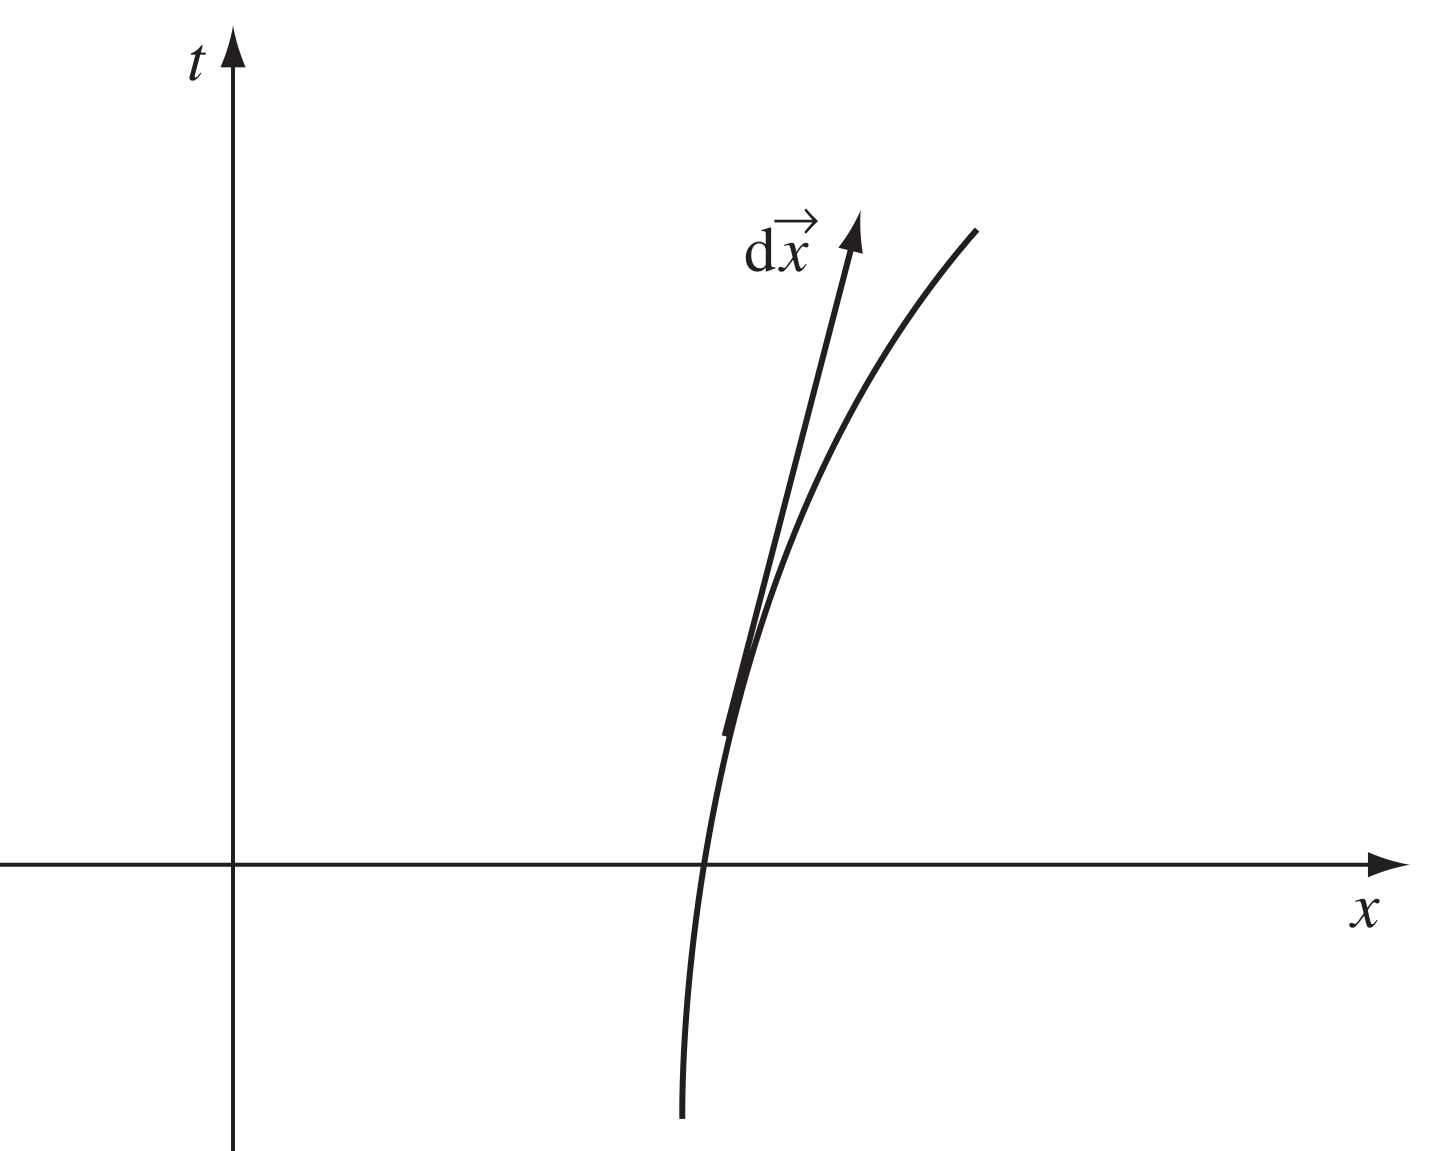
\includegraphics[width=0.6\textwidth]{fig2.5.png}
    \figcaption{\textit{与粒子世界线相切的无穷小位移向量$\rd \vec{x}$.}}
    \label{fig2.5}
}

下面来考虑向量$\rd \vec{x} / \rd \tau$,其中$\rd \tau$等于方程\eqref{equ2.30}的平方根(如图\ref{fig2.5})。这个向量与世界线相切,因为它是$\rd \vec{x}$的倍数。它的模等于
\begin{equation*}
    \frac{\rd \vec{x}}{\rd \tau} \cdot \frac{\rd \vec{x}}{\rd \tau} = \frac{\rd \vec{x} \cdot \rd \vec{x}}{(\rd \tau)^2} = -1.
\end{equation*}
因此它是与世界线相切的、单位模长的类时向量。在MCRF中:
\[
    \rd \vec{x} \xrightarrow[\text{MCRF}, \rd \tau = \rd t]{ } (\rd t, 0, 0, 0).
\]
因此
\[
    \frac{\rd \vec{x}}{\rd \tau} \xrightarrow[\text{MCRF}]{ } (1, 0, 0, 0),
\]
从而有
\[
    \frac{\rd \vec{x}}{\rd \tau} = (\vec{e}_0)_{\text{MCRF}}.
\]
上式右侧就是四维速度的\textit{定义}。由此可得如下的常用表达式:
\begin{shaded}
\begin{equation}
    \vec{U} = \frac{\rd \vec{x}}{\rd \tau}.
\label{equ2.31}
\end{equation}
\end{shaded}

进一步再考虑
\[
    \frac{\rd \vec{U}}{\rd \tau} = \frac{\rd^2 \vec{x}}{\rd \tau^2},
\]
这有一种四维加速度的感觉。我们对方程\eqref{equ2.28}式进行微分,并利用\eqref{equ2.26}式可得
\[
    \frac{\rd}{\rd \tau} (\vec{U} \cdot \vec{U}) = 2 \vec{U} \cdot \frac{\rd \vec{U}}{\rd \tau}.
\]
因为$\vec{U} \cdot \vec{U} = -1$,是个常数,因此
\[
    \vec{U} \cdot \frac{\rd \vec{U}}{\rd \tau} = 0.
\]
由于在MCRF中,$\vec{U}$只有0分量,因此上式的正交性意味着
\[
    \frac{\rd \vec{U}}{\rd \tau} \xrightarrow[\text{MCRF}]{ } (0, a^1, a^2, a^3).
\]
这个向量定义为四维\textit{加速度}向量,记作$\vec{a}$:
\begin{shaded}
\begin{equation}
    \vec{a} = \frac{\rd \vec{U}}{\rd \tau}, \quad \vec{U} \cdot \vec{a} = 0.
\label{equ2.32}
\end{equation}
\end{shaded}
本章习题19说明了为啥叫它“加速度”。

\subsection*{能量与动量}
考虑一个动量为$\vec{p}$的粒子,
\begin{equation}
    \vec{p} \cdot \vec{p} = m^2 \vec{U} \cdot \vec{U} = -m^2.
\label{equ2.33}
\end{equation}
由于
\[
    \vec{p} \cdot \vec{p} = -E^2 + (p^1)^2 + (p^2)^2 + (p^3)^2.
\]
因此
\begin{equation}
    E^2 = m^2 + \sum_{i = 1}^3 (p^i)^2.
\label{equ2.34}
\end{equation}
这是粒子总能量的常用表达式。

某观测者以四速$\vec{U}_{\text{obs}}$运动,他在其中静止的坐标系记作$\MObar$,观者的四速可以不等于粒子四速。
\[
    \vec{p} \cdot \vec{U}_{\text{obs}} = \vec{p} \cdot \vec{e}_{\bar{0}},
\]
其中$\vec{e}_{\bar{0}}$是$\MObar$系的基向量,在该系中粒子四动量的分量为
\[
    \vec{p} \xrightarrow[\MObar]{ } (\bar{E}, p^{\bar{1}}, p^{\bar{2}}, p^{\bar{3}}).
\]
于是,根据\eqref{equ2.26}式可得:
\begin{shaded}
\begin{equation}
    -\vec{p} \cdot \vec{U}_{\text{obs}} = \bar{E}.
\label{equ2.35}
\end{equation}
\end{shaded}
这个结果超级重要。它表明,粒子相对于观测者的能量$\bar{E}$可以在任意坐标系中通过计算标量积$\vec{p} \cdot \vec{U}_{\text{obs}}$得到,这称为相对于观测者的能量的“坐标系无关”的表达式。它在大多数情形下都很有用。

\section{光子}
\label{sec2.7}
\subsection*{光子无四速}
光子在时空图的轨迹是null直线(即切向量都是null向量的直线),即,光子世界线轨迹满足
\begin{equation}
    \rd \vec{x} \cdot \rd \vec{x} = 0.
\label{equ2.36}
\end{equation}
因此$\rd \tau$为零。方程\eqref{equ2.31}表明\textit{光子四速不能定义}。导出该结论的另一种方式是注意到不存在光子在其中静止的坐标系(根据SR的第二个假设),因此光子没有MCRF。所以没有哪个坐标系的$\vec{e}_0$会与光子世界线相切。

注意,仍然可以找到与光子轨迹相切的向量(光子世界线轨迹为直线,它每一点的切向量相等):$\rd \vec{x}$就是一个。问题是找不到\text{单位模长}的切向量,因为所有切向量的模等于零。

\subsection*{四动量}
粒子的四动量\textit{不是}单位向量。粒子四动量在某个坐标系的分量是粒子在那个系中的能量、动量。如果光子在某坐标系中的能量为$E$,则在该系中$p^0 = E$。如果光子在该系中沿$x$轴方向运动,则$p^y = p^z = 0$,由于四动量必须与光子世界线平行,因此光子四动量必须是null向量,从而有$p^x = E$,这保证了
\begin{equation}
    \vec{p} \cdot \vec{p} = -E^2 + E^2 = 0.
\label{equ2.37}
\end{equation}
由此可得,光子\textit{四动量空间部分(spatial momentum)的大小}等于它的能量。

量子力学表明,光子的能量为
\begin{equation}
    E = h\nu,
\label{equ2.38}
\end{equation}
其中$\nu$是光子频率、$h$是Planck常量,$h = 6.6256 \times 10^{-34} \, \mathrm{J \, s}$。

这个关系式结合四动量的Lorentz变换可以得到光子的Doppler频移公式。例如,某个光子在$\MO$系中的频率为$\nu$,沿$x$方向运动。则在$\MObar$系中(它相对于$\MO$系沿$x$轴以速度$v$运动)的光子能量为:
\begin{align*}
    \bar{E} &= \frac{E}{\sqrt{1 - v^2}} - \frac{p^x v}{\sqrt{1 - v^2}} \\
    &= \frac{h \nu}{\sqrt{1 - v^2}} - \frac{h\nu v}{\sqrt{1 - v^2}}.
\end{align*}
结合$\bar{E} = h\bar{\nu}$可得到光子在$\MObar$系中的频率的关系:
\begin{equation}
    \frac{\bar{\nu}}{\nu} = \frac{1 - v}{\sqrt{1 - v^2}} = \sqrt{ \frac{1 - v}{1 + v} }.
\label{equ2.39}
\end{equation}
一般情况的频移公式见本章习题25.

\subsection*{静质量为零的粒子}
光子的静质量为零,因为:
\begin{equation}
    m^2 = -\vec{p} \cdot \vec{p} = 0.
\label{equ2.40}
\end{equation}
四动量为null向量的\textit{任意}粒子静质量必然为零,反之亦然。目前已知静质量为零的唯一粒子是光子。中微子很轻,但并非无质量。\textit{(有时无质量粒子也包括“引力子”,因为后面会看到,引力波以光速传播。但是“光子”与“引力子”都是来自量子力学的概念,而目前没有合适的引力量子化理论,因此“引力子”还不是一个有良好定义的概念。)} 将有限大小静质量的粒子加速到光速需要无穷大的能量,因此只有静质量为零的粒子才能以光速运动。另一种说明方法是,一个以光速运动的粒子(简明起见设它沿$x$方向运动)满足$p^1 / p^0 = 1$,而静质量为$m$、沿$x$轴运动的粒子,根据$\vec{p} \cdot \vec{p} = -m^2$,有$p^1 / p^0 = \big[ 1 - m^2 / (p^0)^2 \big]^{1/2}$,无论给该粒子多少能量,这个比值总是小于1。尽管可以让静质量非零的粒子无限接近光速,但存在着质的不同:$m \neq 0$的粒子总是有MCRF——即粒子在该系中静止的Lorentz系(惯性系),它相对于旧坐标系的速度$v = p^1 / p^0$. 而光子\textit{没有}静止坐标系。


\section{扩展阅读}
\label{sec2.8}
本章简要阐述了相对论运动学及粒子动力学的内容。它们在粒子物理学中特别重要,这也为SR提供了最严格的检验。详见Hagedorn (1963) 或者 Wiedemann (2007)。

\section{习题}
\label{sec2.9}